\section{Background and Motivation}
\label{sec:background}
\subsection{GPU Systems and Workload Diversity}
\label{sec:arch-gpu}

% \arq{I think this is too many ideas for one paragraph  It should probably reference Figure 1 (!)}
As shown in \Cref{fig:motivation_silos}, we focus on three GPU resource management domains across the software stack: memory placement and migration, compute scheduling, and on-device thread scheduling. User-space frameworks (e.g., vLLM~\cite{kwon2023efficient}, Salus~\cite{yu2020fine}, PILOT~\cite{ravi2021pilot}) leverage application semantics (e.g., neural structures, latency constraints) to implement request scheduling and KV-cache offloading policies. Kernel drivers manage memory, scheduling, and multi-tenant isolation via privileged hardware mechanisms (MMU, interrupts), typically using fixed, application-agnostic algorithms (e.g., LRU eviction) under Unified Virtual Memory (UVM), which transparently handles oversubscription through host-device page migrations. GPU devices execute kernels via SIMT (Single Instruction, Multiple Threads); on NVIDIA hardware, 32-thread warps run instructions in lockstep on SMs, with internal states (e.g., warp access patterns) opaque to host drivers.


\begin{figure}[t]
    \centering
    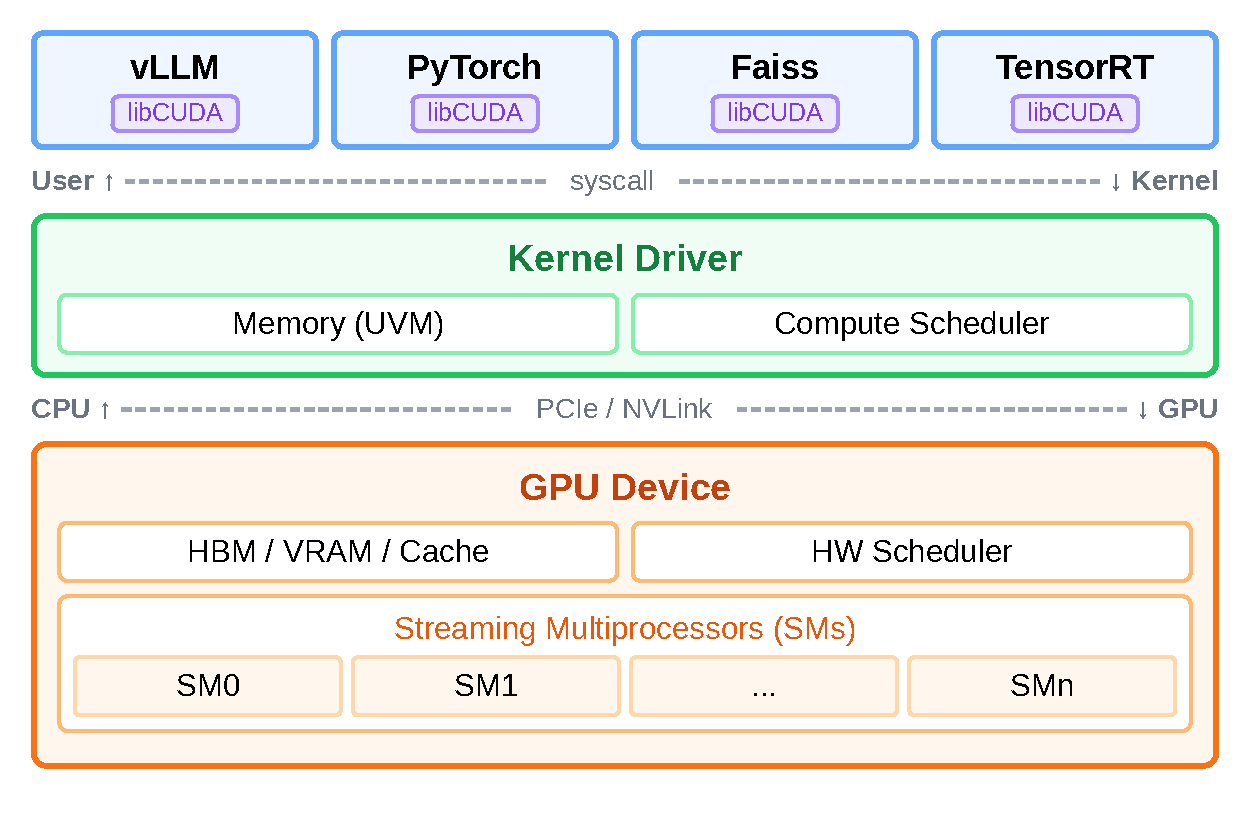
\includegraphics[width=\columnwidth]{img/gpu_stack_figure.pdf}
    \caption{GPU system stack: user-space frameworks, kernel driver (memory and scheduling), and GPU hardware.}
    \label{fig:motivation_silos}
\end{figure}

% \arq{I think this should be two paragraphs: one that talks about workload diversity and the second that then talks about the need for different policies.}
GPU workloads exhibit diverse resource access patterns. Results from \sys{}'s eBPF-based tracing tools (\S\ref{sec:eval}) confirm this diversity: \Cref{fig:access_patterns} captures memory page-fault addresses over time under UVM, showing that LLM MoE inference exhibits periodic stride bursts from expert activations; GNN training shows irregular random access from pointer-chasing graph traversal; and vector search alternates between sequential scans (index build) and random probes (query)~\cite{pan2024survey,cao2023gpu}. \Cref{fig:thread_scheduling} reveals a 127$\times$ SM scheduling load imbalance in a vector-add GPU kernel, invisible to host-side drivers.

These diverse patterns require workload-specific policies across all three domains. UVM eviction and prefetch policies alone can impact execution time by up to 73\%~\cite{ganguly2019interplay,park2025helm}: MoE inference favors specialized eviction over default LRU~\cite{sheng2023flexgen,kwon2023efficient}, while GNN training demands aggressive sequential prefetch~\cite{lin2024towards,wang2016gunrock}, but each can degrade other workloads. Compute scheduling requires adaptive priority and preemption policies as multi-tenant demands fluctuate~\cite{fan2025gpreempt,wang2024gcaps}, and SM load imbalance benefits from custom thread scheduling. Yet current drivers and firmware enforce a single fixed policy.
\begin{figure*}[t]
    \centering
    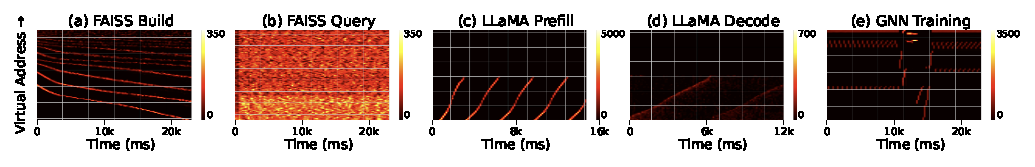
\includegraphics[width=\textwidth]{img/pattern/combined_patterns_1x5_v2.pdf}
    \caption{Page-fault address traces over time across four workloads. Each pattern implies a different optimal prefetch/eviction strategy; no single policy fits all.}
    \label{fig:access_patterns}
\end{figure*}


\begin{figure}[t]
    \centering
    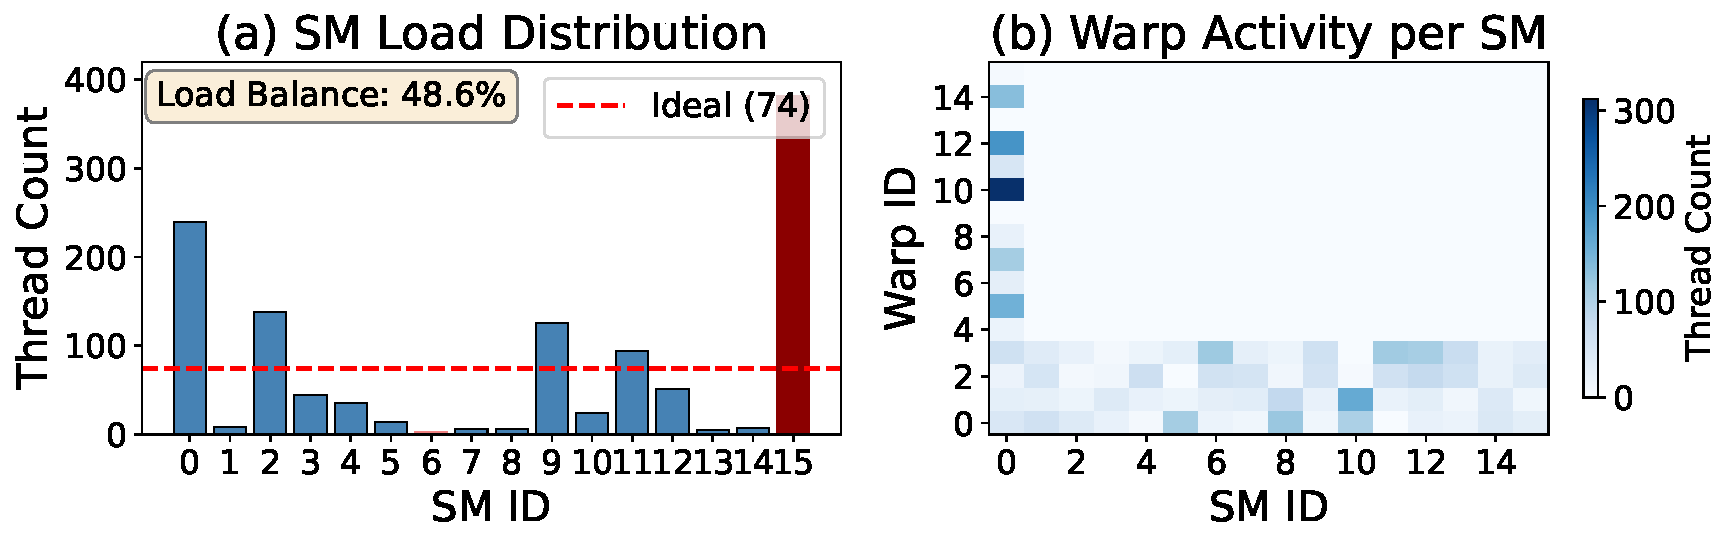
\includegraphics[width=\columnwidth]{img/pattern/vector_add/thread_scheduling_motivation.pdf}
    \caption{GPU thread scheduling imbalance observed via eBPF tracing. (a) SM load distribution: 127$\times$ imbalance. (b) Warp activity heatmap across SMs.}
    \label{fig:thread_scheduling}
\end{figure}

\subsection{Agent-Based Policy Exploration}
\label{sec:motivation-agent}

Agentic OS policy exploration fits the large GPU policy space but requires programmable interfaces at the relevant control boundaries. Unlike parameter-tuning methods, AI agents~\cite{dwivedula2025policysmith,zheng2025schedcp} directly generate and iteratively refine policy logic to explore richer, workload-specific strategies. Ordinary driver/UVM interfaces expose preset controls (e.g., \texttt{cudaMemAdvise}, driver module parameters), rather than arbitrary workload-aware eviction or fault-path prefetch callbacks. Framework and driver extensions can add programmability, with the boundaries discussed below.

Effective GPU policy optimization requires an OS interface with three key properties: (1) \emph{safe}, robustly handling generated policies without kernel panics or GPU corruption; (2) \emph{dynamic}, rapidly deploying and iterating policies at runtime without application restarts or kernel rebuilds; and (3) \emph{full-stack}, observing GPU-internal states, coordinating across tenants, and controlling driver-level decisions like eviction and fault-path prefetching.

\subsection{Limitations of Existing Approaches}
\label{sec:motivation-limitations}

% \arq{Make sure to critique these existing approaches by saying they are not safe, dynamic, or full-stack.}
Existing approaches fail to simultaneously provide a safe, dynamic, and full-stack programmable OS interface for GPU resource management.

\paragraph{Driver-Level Policies}
Driver-level approaches expose preset controls (e.g., \texttt{cudaMemAdvise} and driver module parameters) or add custom control paths. Systems like TimeGraph~\cite{kato2011timegraph}, Gdev~\cite{kato2012gdev}, and OS kernel interception methods~\cite{kernelintercept} embed scheduling or memory-management logic into driver modules. More recent work such as GPREEMPT~\cite{fan2025gpreempt} and GCAPS~\cite{wang2024gcaps} adds priority-based preemption, while LithOS~\cite{coppock2025lithos} provides a redesigned runtime. These systems have different trust and deployment boundaries; a modified driver is not inherently an unsafe implementation. The relevant distinction is whether a policy can change independently of trusted driver code, and which observations and actions its interface exposes. \Cref{tab:policy-expressibility} identifies those boundaries for the policies considered here.

\paragraph{Host User-Space Runtimes and Libraries}
User-space frameworks~\cite{ng2023paella,gim2025pie,shen2025xsched,chen2025ktransformers,coppock2025lithos} can implement rich policies when applications expose the necessary state and controls. Framework integration supplies useful semantics but can require per-framework adapters. A shared user-space scheduler can coordinate participating tenants~\cite{xiao2018gandiva,yu2020fine}; process boundaries do not make such coordination impossible. Ordinary application APIs do not, however, place arbitrary policy code inside a UVM fault handler or expose PMM eviction-list transitions. Device-side instrumentation and cooperating kernels provide other observations and controls, with their own integration requirements. Our comparison therefore concerns specific missing control boundaries, not a blanket inability of user space to schedule across tenants or observe GPU execution.
